\documentclass[a4paper]{report}
\usepackage[14pt]{extsizes}
\usepackage[utf8]{inputenc}
\usepackage[english,russian]{babel}
\usepackage[OT1]{fontenc}
\usepackage{setspace, amsmath}
\usepackage{amsfonts}
\usepackage{amssymb}
\usepackage[left=20mm, top=10mm, right=15mm, bottom=20mm, nohead, footskip=10mm]{geometry}
\usepackage{gensymb}

\usepackage{graphicx} 
\graphicspath{{images/}}
\DeclareGraphicsExtensions{.pdf,.png,.jpg}

\renewcommand{\theenumi}{\arabic{enumi}}
\renewcommand{\labelenumi}{\arabic{enumi}}
\renewcommand{\theenumii}{.\arabic{enumii}}
\renewcommand{\labelenumii}{\arabic{enumi}.\arabic{enumii}.}
\renewcommand{\theenumiii}{.\arabic{enumiii}}
\renewcommand{\labelenumiii}{\arabic{enumi}.\arabic{enumii}.\arabic{enumiii}.}
\usepackage{indentfirst}
\usepackage{fontspec}
\setmainfont{Times New Roman}

\begin{document}
\begin{titlepage}
\newpage



\begin{center}
\vfill
%\framepage

Федеральное государственное бюджетное образовательное учреждение высшего образования «МИРЭА — Российский технологический университет»\\
\ \\

\hfill\vbox
{
\hbox{Кафедра высшей математики}
}

\vfill

{\large\bf Разработка безопасного аудиокодека с шифрованием трафика\\}
\ \\
Реферат студентов 1 курса института искусственного интеллекта\\
Коровяковского Степана и Урвачева Романа

\vfill

%{
%\hbox{Научный руководитель:}
%\hbox to 16cm {к.т.н, доцент \hrulefill Х.З.~Мамаев}
%\hbox{}
%\hbox{Заведующий кафедрой:}
%\hbox to 16cm {д.ф.-м.н., профессор \hrulefill В.С.~Луговской}
%}

\vfill

Москва 2022
\end{center}

\end{titlepage}
\tableofcontents
\newpage
\chapter*{Введение}
\chapter{Изучение способов передачи аудиоданных в информационно-телекоммуникационных сетях}
\section{Телекоммуникационные технологии}
Каждому поколению свойственно разрабатывать новые технические средства, совершенствовать систему учета, обработки, передачи и хранения данных. Первыми телекоммуникационными средствами признан телеграф, телефон, телетайп, радиоприемник. Середина XIX столетия отмечена массовым использованием спутниковой связи, вычислительной техники, компьютерной сети. В результате это положительно отразилось на развитии новых телекоммуникационных технологий.
\par Современный мир невозможен без телекоммуникационных технологий, которые стирают государственные границы и расстояние между людьми, делают доступной мобильную и видеосвязь и позволяют решать множество задач в сфере управления, образования, коммерции. Каждый человек сталкивается с ними ежедневно, деля телефонные звонки, проверяя почту или покупая товары в интернет-магазинах.

\subsection{Определение и понятие телекоммуникационных \\ технологий}
Общее понятие информационных и коммуникационных технологий включает в себя совокупность методов, процессов и устройств, позволяющих получать, собирать, накапливать, хранить, обрабатывать и передавать информацию, закодированную в цифровом виде или существующую в аналоговом виде.
\par В более узком смысле под телекоммуникационными технологиями понимается совокупность программных и аппаратных средств, позволяющих устанавливать связь без использования проводов и передавать пакеты информации.

\subsection{Виды телекоммуникационных технологий}
Телекоммуникационные технологии могут быть рассмотрены как сервисы, предоставляемые провайдерами различного уровня.
По этому принципу можно выделить следующие виды телекоммуникационных технологий:
\begin{itemize}
\item телефонная связь, современная телефонная связь позволяет легко переключаться с аналогового стандарта на цифровой, подключать к интернет городские телефоны и соединять в одну сеть аналоговые и мобильные устройства;
\item радиосвязь, которая сегодня превратилась в сотовую связь, телефон, перемещаясь в пределах сети, оказывается в зоне действия различных передающих устройств;
\item спутниковая связь, которая используется провайдерами для создания систем мобильной связи и для государственных систем связи;
\item интернет – наиболее распространенный вид телекоммуникационных технологий, при которых подключение к сети может осуществляться как проводным, так и беспроводным способом.
\end{itemize}

\subsection{Основные типы информационно-телекоммуникационных сетей}
Телекоммуникационные технологии, используемые в интернете, сейчас переживают этап бурного развития и роста. С каждым днём создаётся всо больше и больше новых сетей различных типов, среди которых основными являются:
\begin{itemize}
\item локальные сети компаний или учреждений (Local Area Network - LAN), связь между компьютерами в них осуществляется и проводным и беспроводным способом, количество пользователей этих сетей ограничено. Локальные сети могут быть корпоративными, в некоторых странах создаются и городские локальные сети;
\item глобальные сети (Wide Area Network – WAN) представляют совокупность большого количества узлов-компьютеров, расположенных в разных странах мира и связанных между собой каналами оптово-волоконной связи. К этим сетям, представляющим услуги провайдеров, подключаются локальные сети.
\end{itemize}

\subsection{Технические и программные средства \\ телекоммуникационных технологий}
Работоспособность интернета основана на использовании сетевых узлов и каналов связи. К узлам относятся как отдельные компьютеры, так и хостинги, предоставляющие IP-адреса и доменные имена.
Каналы связи делятся на 4 типа:
\begin{itemize}
\item аналоговые телефонные сети;
\item провода, по которым передается электричество;
\item оптоволоконные каналы связи;
\item беспроводные каналы связи, модемные или спутниковые.
\end{itemize}
К телекоммуникационным каналам связи относятся, в основном, третий и четвертый типы.

Среди коммуникаций, используемых для организации связи, можно отдельно отметить программы, обеспечивающие работу телекоммуникационного оборудования такого, как:
\begin{itemize}
\item IP-АТС;
\item маршрутизаторы;
\item компьютеры.
\end{itemize}

\subsection{Программное обеспечение телекоммуникационных \\ технологий}
Для передачи данных с использованием возможностей телекоммуникационных технологий применяется специальное программное обеспечение. Это обеспечение функционирует по определенным протоколам или по механизмам, разработанным с целью упростить и стандартизировать работу всех узлов сети, выстроив ее по единому алгоритму.

Так, для передачи по компьютерным сетям разработан стандарт MIME (ssr-Multipurpose Internet Mail Extensions), переводящий данные в формат понятный почтовому серверу. Общение компьютера пользователя и сервера происходит в виде диалога в режиме Клиент-Сервер, где с каждой стороны его участником является определенная программа.

Отдельные программы используются для работы мессенджеров, которые позволяют обмениваться сообщениями, совершать телефонные звонки с передачей голосовой и видеоинформации. Здесь происходит коммуникация не только компьютер - почтовый сервер, к диалогу подключаются и телефонные станции.

\subsection{Основные задачи сетевых телекоммуникационных технологий}
Различные сетевые телекоммуникационные технологии позволяют решать такие задачи, как:
\begin{itemize}
\item передачу информации в необходимых форматах;
\item выстраивание коммуникаций;
\item обеспечение взаимодействия различных участников сети.
\end{itemize}

Среди новых технологий особое место занимают программы, позволяющие работать в режиме нетворкинга, объединение CRM-систем с возможностями социальных сетей и многое другое.

Создание корпоративных сетей как офисных, компьютерных, так и телефонных, также попадает в область сетевых технологий, призванных обеспечить синергию за счет эффективной коммуникации пользователей.

\subsection{Технологии защиты информации в телекоммуникационных сетях}
Большая часть информационных массивов, принадлежащих государственным учреждениям и коммерческим предприятиям, имеет самостоятельную ценность и является добычей для потенциальных похитителей, которыми могут быть и хакеры, и внутренние пользователи.

Для защиты информации от утечек разработаны сложные программные продукты, позволяющие определить проникновение неавторизованного пользователя или вируса-похитителя информации в сеть и блокировать его.

Существуют специальные стандарты защиты информации, но даже они не всегда могут уберечь сети от взлома и хищения данных. Особенно уязвимы компьютеры и мобильные устройства частных пользователей, использующих только антивирусы.

От хищения информации с помощью закладных устройств, перехватывающих электромагнитные излучения, необходимо бороться при помощи технических средств.

\subsection{Использование телекоммуникационных технологий}
Телекоммуникационные технологии сегодня в основном применяются для организации систем связи.

Но сами системы связи имеют прикладное значение, при помощи этих технологий можно достичь существенно более важных целей, среди которых:
\begin{itemize}
\item создание систем дистанционного обучения;
\item обеспечение недорогой голосовой телефонной связи;
\item создание информационных систем предприятий и объединение их в комплекс, позволяющий оптимизировать управление;
\item построение банковских сетей;
\item проведение электронных аукционов и тендеров для обеспечения государственных закупок;
\item осуществление коммуникации удаленных субъектов;
\item для интернет-торговли;
\item осуществление дистанционного управления в государственной и в частной сфере.
\end{itemize}

Спектр возможностей использования телекоммуникационных технологий расширяется с каждым днем. Сложно сказать, что именно будет предложено завтра в этой области, чтобы сделать связь доступнее, а производственные процессы – проще.

\section{Описание способов передачи аудиоданных}
\subsection{Передача аудиоданных по телефонным каналам связи}

Взаимное проникновение вычислительной техники и технических средств связи оказало серьезное влияние как на структуру компьютеров, так и на структуру каналов связи.

Средства связи, предназначенные для передачи информации между людьми, имеют длительную историю, развитую структуру (в мировом масштабе), мощную научную и технологическую базу и, начиная с 60-х годов, стали использоваться для передачи данных, т.е. для передачи информации между техническими средствами вычислительной техники, что потребовало включения в каналы связи дополнительных технических ус тройс тв.

В настоящее время для распределенных вычислительных систем наиболее широко используются телефонные каналы.

На рис. 1.2.1.1 представлена упрощенная схема линии аналоговой междугородней телефонной связи.

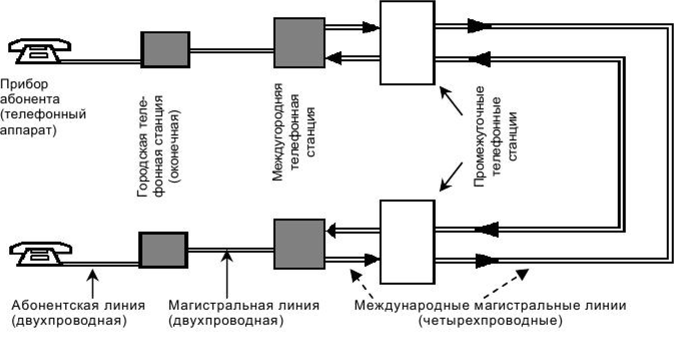
\includegraphics[scale=1.4]{66}
{\centering\caption{Рис. 1.2.1.1 Схема междугородней телефонной связи}\\}
~

На участке от телефонного аппарата до местной АТС происходит передача в первичной полосе частот « 200 - 3100 Гц (полоса частот человеческого голоса). При этом от каждого аппарата до АТС проводится двухпроводная электрическая линия для передачи этого сигнала, в дальнейшем происходит преобразование его в иную форму с целью уплотнения передачи. В каждом из последующих каналов идет очень большое количество передач. Существует два типа уплотнения: частотное и временное. В традиционных линиях связи, как правило, используется частотное уплотнение.

Сущность частотного уплотнения для грех абонентов представлена на рис. 1.2.1.2.

\bigskip
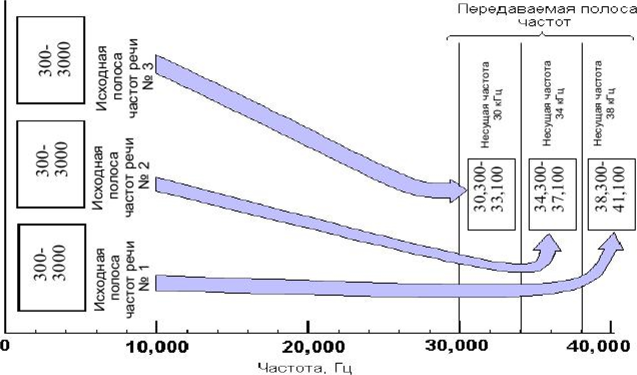
\includegraphics[scale=1.4]{67}
{\centering\caption{\newline Рис. 1.2.1.2 Частотное уплотнение телефонных каналов}\\}
~

Передаваемый сигнал на входе в магистральную линию «смешивается» с так называемой несущей (более высокой) частотой и одновременно с другими сигналами (которые передаются на других несущих частотах) распространяется по магистралям. На выходе передаваемые сигналы выделяются из несущих частот и по индивидуальным линиям доставляются абоненту.

Процедура на входе в магистральные линии связана с различного вида модуляцией несущих частот, а обратное преобразование на выходе из магистральных линий, соответственно, с демодуляцией.

Модуляция несущей - изменение ее амплитуды, частоты, фазы или комбинации этих характеристик в соответствии с передаваемым сигналом.

Использование описанных средств связи для передачи данных, т.е. замена абонента-человека на техническое устройство (ЭВМ), требует включения в эту систему дополнительных устройств, адаптирующих информационные СОД к передаче по каналу связи.

\newpage
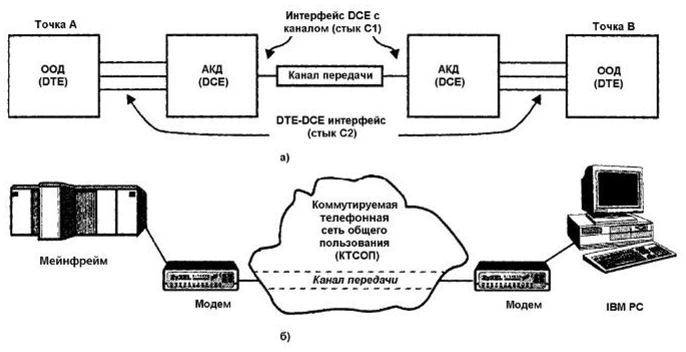
\includegraphics[scale=1.4]{68}
{\centering\caption{\newline Рис. 1.2.1.3 Типовая схема передачи данных: а - блок-схема системы передачи данных; б - реальная система передачи данных}\\}

~

На рис. 1.2.1.3, а) приведены традиционно используемые сокращения для обозначения устройств систем передачи данных (СПД):

ООД - оконечное оборудование данных, в качестве которого может выступать персональный компьютер, большой компьютер, терминал и т.п. В литературе часто употребляется международный термин DTE (Data Terminal Equipment);

АКД - аппаратура канала данных, которую иногда называют аппаратурой передачи данных (АПД), функции которой состоят в обеспечении возможности передачи информации по каналу определенного типа, эти устройства, как правило, называются модемами (модулятор-демодулятор); DCE (Data Communications Equipment) - международный термин, используемый для обозначения этого \\ устройства.

Канал передачи включает описанную выше структуру, если используется коммутируемая телефонная сеть общего назначения.

Интерфейс между каналами передачи и АКД в отечественной практике называется «стык 1» (С1), а интерфейс между ООД и АКД «стык 2» (С2).

\subsubsection{Описание типов каналов связи}

В зависимости от типа передачи различают аналоговые (традиционно используемые, имеющие длительную историю развития) и цифровые каналы (систем ИКМ, ШОЫ и др.), являющиеся битовым трактом с цифровым импульсным сигналом на выходе и входе канала. Цифровые каналы отличаются рядом преимуществ перед аналоговыми, поэтому вновь создаваемые системы передачи данных стараются строить на основе цифровых каналов. Следует отметить, что цифровые каналы весьма успешно применяются не только для передачи данных, но и в средствах бытовой связи (звук, изображение и г.д.), при этом аналоговые сигналы кодируются в цифровые перед передачей в канал.

Термины «аналоговый» и «цифровой» соответствуют непрерывным и дискретным процессам и используются при обсуждении коммуникационных систем в различных контекстах - данных, сигналов и передачи.

Аналоговые данные представляются физической величиной, которая может изменяться в непрерывном диапазоне значений. Величина прямо пропорциональна данным или является их функцией.

Цифровые данные принимают дискретные значения - текст, целые числа, двоичные данные.

Аналоговый сигнал - непрерывно изменяющаяся электромагнитная волна, распространяющаяся в различных средах.

Цифровой сигнал - дискретный (разрывной) сигнал, такой, как последовательность импульсов напряжения.

Возможны четыре вида передачи данных:
\begin{enumerate}
\item) цифровые данные - цифровой сигнал, используется наиболее простое оборудование;
\item) аналоговые данные - цифровой сигнал, необходимо преобразование аналоговых данных в цифровую форму, что позволяет использовать современное (высокоэффективное) оборудование передачи данных;
\item) цифровые данные - аналоговый сигнал, необходимость преобразования связана с тем, что через некоторые среды (оптоволокно, беспроводные среды) может распространяться только аналоговый сигнал;
\item) аналоговые данные - аналоговый сигнал, традиционная передача, аналоговые данные легко преобразуются в аналоговый сигнал.
\end{enumerate}

Среди преимуществ цифровой передачи необходимо отметить следующие.
\begin{itemize}
\item \qquad Быстрое развитие цифровых систем и уменьшение цены и размеров оборудования, цены и размеры аналогового оборудования остаются на прежнем уровне. Обслуживание цифровых систем намного дешевле аналоговых.
\item \qquad Использование повторителей (в цифровых системах) вместо аналоговых усилителей позволяет передавать данные на большие расстояния по менее качественным линиям (нет накопления шумов) - сохранение целостности данных.
\item \qquad Большая пропускная способность дает возможность более полно использовать пропускную способность оптоволокна и спутниковых средств связи. Временное разделение оказывается более эффективным, чем частотное.
\item \qquad Используется интеграция, когда при обработке аналоговой и цифровой информации по цифровым технологиям все сигналы имеют одинаковую форму (вид). Эго позволяет сэкономить на оборудовании и трудозатратах при интеграции: голос, видео, цифровые данные.
\end{itemize}

Термин «модем» (ЭСЕ) применяется в настоящие время (в связи с распространением цифровых каналов) достаточно широко, при этом необязательно подразумевается какая-либо модуляция, а просто называются определенные операции преобразования сигналов, поступающих от ЭТЕ для их дальнейшей передачи по используемому каналу.

Существует очень много разновидностей модемов, отличающихся:
\begin{itemize}
\item по конструкции - внутренние (вставляемые в разъемы компьютера) и внешние, портативные, групповые и т.н.;
\item по методу передачи - асинхронные, синхронные, синхронноасинхронные.
\end{itemize}

Асинхронный метод передачи (или стартстопный) - посимвольный режим передачи с контролем начала и конца символа, имеет низкую скорость и малую эффективность. Синхронный метод передачи осуществляет объединение большого количества символов или байт в отдельные блоки - кадры, которые передаются без задержек между восьмибитными элементами.

~

Очень важной характеристикой канала передачи являются режимы его работы в зависимости от направления возможной передачи данных:
\begin{itemize}
\item симплексный - передача осуществляется по линии связи только в одном направлении;
\item полудуплексный - передача ведется в обоих направлениях, но попеременно во времени (технология Ethernet);
\item дуплексный - передача ведется одновременно в двух направлениях.
\end{itemize}

Дуплексный режим - наиболее универсальный и производительный. Самым простым вариантом организации дуплексного режима является использование двух независимых функциональных каналов (двух пар проводников или двух световодов) в кабеле, каждый из которых работает в симплексном режиме, т.е. передает данные в одном направлении. Такая организация дуплексного режима применяется во многих сетевых технологиях (Fast Ethernet, ATM и т.п.).

\subsubsection{Способы повышения эффективности передачи данных}

Существует два основных способа повышения эффективности.

Первый способ, о котором уже упоминалось, - уплотнение информации (или в современной терминологии - мультиплексирование), г.е. функция, позволяющая двум или более источникам данных совместно использовать общую среду передачи данных таким образом, что каждый получает собственный канал передачи данных.

Традиционным считается частотное мультиплексирование, о котором достаточно подробно говорилось ранее, - разделение системы передачи на два или более канала путем разделения всей доступной полосы частот на более узкие полосы, каждая из которых образует отдельный канал.

Второй тип - временное мультиплексирование, интенсивное внедрение которого связано с современным развитием систем передачи на два или более канала путем поочередного подключения общей линии к разным информационным каналам. Распространению временного мультиплексирования способствовало значительное увеличение пропускной способности каналов, поскольку чем выше пропускная способность канала, тем больше эффективность временного мультиплексирования.

Различают синхронное временное мультиплексирование - методика временного мультиплексирования, когда порядок выделения временных интервалов жестко задан, в отличие от статистического (асинхронного) временного мультиплексирования, при котором временные интервалы, на которые общая линия выделяется устройством, а также порядок их выделения не определены заранее (определяется динамически).

Частотное мультиплексирование - разделение системы передачи на два или более канала путем разделения всей доступной полосы частот на более узкие полосы, каждая из которых образует отдельный канал.

Общий случай частного мультиплексирования иллюстрирует рис. 1.2.1.4, а. Шесть источников сигналов подключены к мультиплексору, который модулирует каждый сигнал определенной частотой. Для передачи каждого сигнала требуется полоса частот, центр которой находится вблизи несущей частоты. Эта полоса частот обычно называется каналом. С целью предотвращения перекрестного шума каналы разделяются защитными полосами, которые не используются для передачи информации.

~

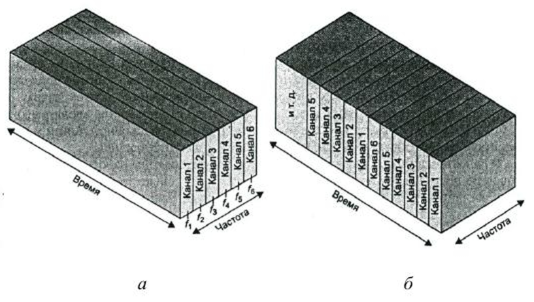
\includegraphics[scale=1.6]{69}
{\centering\caption{\newline Рис. 1.2.1.4 Частотное (а) и временное (б) мультиплексирование }\\}

~

Сигнал, передаваемый по среде передачи, является аналоговым. Однако входные сигналы могут быть как цифровыми, так и аналоговыми. В случае цифровых сигналов их необходимо пропустить через модемы для преобразования в аналоговую форму. В любом случае должен модулироваться для сдвига в необходимую полосу частот.
\newpage
Временное мультиплексирование - разделение системы передачи на два или более канала путем поочередного подключения общей линии к разным информационным каналам.

Временное мультиплексирование становится возможным, когда скорость распространения сигналов в среде превышает скорость их передачи. В таком случае ряд цифровых или аналоговых сигналов может передаваться одновременно путем поочередной передачи «порции» каждого сигнала. Общий случай временного мультиплексирования показан на рис. 4.4, 6. Шесть источников ситналов подключены к мультиплексору, который чередует биты сигналов, поочередно передавая информацию от каждого из источников. Этот мультиплексор обладает шестью входами. Если каждый из них может поддерживать скорость передачи данных, скажем,
9.6 Кбит/с, тогда единая линия пропускной способностью 57.6 Кбит/с будет передавать сиг налы сразу от всех шести источников.

~

Второй способ повышения эффективности использования среды передачи данных - компрессия или сжатие данных, заключающееся в уменьшении количества битов, требуемых для представления данного объема информации. Это позволяет увеличить объем информации, передаваемой по линии, сократить сеанс связи, кроме этого кодирование информации, связанное с компрессией, повышает информационную безопасность.

\subsection{Передача аудиоданных по радиосвязи}

\subsubsection{Распространение радиоволн, расстояние и длина волны}

Передача аудиоданных по радиосвязи осуществляется путём распространения радиоволн. Радиоволны распространяются в пространстве различным образом. Способ их движения в первую очередь зависит от их длины. Так, например, волны от 10 км и выше (сверхдлинные – СДВ) без труда огибают наземные препятствия как искусственного, так и естественного происхождения. Они теряют мало энергии в процессе своего распространения и затухают гораздо медленнее, чем волны других длин. По этой причине они могут перемещаться в пространстве на тысячи километров. Также они обладают высокой степенью проникновения в среду, поэтому их широко используют для исследований земной коры для нужд археологии, геологии, инженерного дела. Их применяют для исследования атмосферы планеты. Также с их помощью осуществляют связь с подводными объектами.

Километровые волны также называют «длинные» (ДВ), они составляют 1-10 км и тратят больше энергии при распространении, способны покрывать расстояния до 2000 км. Близкий к ним тип – средние (СВ) от 100 м до 1 км. Они сильнее поглощаются земной поверхностью, поэтому имеют еще меньший диапазон распространения – порядка 1000 км.

Короткие волны (КВ – 10-100 м) распространяются не далее чем на 250 км, однако обладают интересным свойством. Часть их, уходящая под большим углом к горизонту, соприкасаясь с верхними слоями атмосферы (ионосферой) отражается и направляется обратно к поверхности. Затем они снова отражаются, теперь уже от земли и снова направляются вверх. Распространяясь таким образом короткие волны могут несколько раз обойти вокруг планеты. Ионосфера теряет свою отражательную способность в ночное время, поэтому связь на коротких волнах в это время суток будет хуже.

Длина ультракоротких волн (УКВ) составляет от 1 см до 10 м, к ним относятся метровые (МВ), дециметровые (ДМВ), сантиметровые (СМВ). Они успешно преодолевают ионосферу не отражаясь от нее. Они уходят выше и применяются для исследования свойств облаков, наблюдения за птицами, определения координат самолетов. Но так как отсутствует эффект отражения, они не могут огибать планету и радиосвязь с их помощью ограничена расстоянием в 200-300 км. С помощью специальных антенн УКВ собирают в «пучок», усиливают и отправляют в указанном направлении, что широко используется при обеспечении спутниковой связи, а также в радиолокации.

Миллиметровые волны (ММВ) во многом схожи с УКВ, однако для них серьезной помехой служат атмосферные явления, такие как дождь, снег, туман, облака. За счет ММВ обеспечивается работа высокоскоростной радиорелейной связи. Они нашли свое применение в быту, их используют в медицине, они пригодились в радиоастрономии.

\subsubsection{Оборудование применяемое для передачи радиоволн}

Радиосвязь – быстрый и относительно надежный способ передачи данных на большие расстояния. При этом нет необходимости в использовании физического носителя, например проводов.

Свойства волн разной длины напрямую влияют на их применение для обеспечения радиосвязи. Кроме того, на качество передачи информации с их помощью влияют следующие факторы:

\begin{itemize}
\item высота приемной и передающей антенн;
\item рельеф поверхности;
\item солнечная активность, метеоусловия, время суток.
\end{itemize}

Процесс приема-передачи информации с помощью радиоволн состоит из следующих основных этапов:

\begin{enumerate}

\item) формирование сигнала;
\item) выделение несущей частоты;
\item) связывание передаваемой информации с несущей частотой (модуляция);
\item) трансформация сигнала в дискретный вид, его кодирование (для цифровых систем);
\item) передача в радиоэфир с помощью антенны;
\item) прием сигнала;
\item) декодировка и демодуляция;
\item) преобразование сигнала в форму понятную абоненту.
\end{enumerate}

Чтобы реализовать обмен информации необходимо чтобы у принимающей и передающей стороны в наличии было следующее оборудование:

\begin{itemize}
\item передатчик;
\item антенна;
\item ретрансляционное устройство – позволяет увеличить дальность передачи сигнала;
\item принимающее устройство;
\item оборудование модуляции-демодуляции, сжатия, оцифровки и кодирования;
\item фильтры помех, усилители.
\end{itemize}

Две простейшие радиостанции, как правило, могут обмениваться информацией на очень небольших расстояниях. Чтобы значительно увеличить зону покрытия, необходимо использовать один из следующих методов:

\begin{itemize}
\item сеть ретрансляторов, установленных на поверхности планеты;
\item орбитальные спутники;
\item системы передвижной радиосвязи.
\end{itemize}

Применяется несколько способов радиосвязи, для каждого из которых используется специфическое оборудование. Три наиболее распространенных вида:
\begin{itemize}
\item сотовая связь;
\item радиорелейная связь;
\item спутниковая связь.
\end{itemize}

\subsubsection{Сотовая связь}

При ее использовании сигнал идет от передатчика к приемникам, расположенным на одинаковом расстоянии друг от друга. Они образуют гексагональную фигуру, которую называют «сота». Такое построение сети позволяет обеспечить в области покрытия высокое качество сигнала, которое будет определяться количеством приемников расположенных рядом с местом приема или передачи. В настоящее время этот вид связи является наиболее популярным и чаще всего используемым. Роль приемника и передатчика здесь играет персональный телефонный аппарат. Основное преимущество сотовой связи – обеспечение высокой мобильности абонента.

\subsubsection{Радиорелейная связь}

Вид радиосвязи, осуществляемой с помощью цепочки передающих станций, находящихся в прямой видимости их антенн. Работают в дециметровом и сантиметровом диапазонах. Возможна одновременное функционирование большого количества передатчиков. Уровень индустриальных и атмосферных помех радиоприему в ДМ и СМ диапазонах низкий. Главный недостаток – ограниченное расстояние передачи и высокая степень зависимости от коммуникационной инфраструктуры – сети ретрансляторов.

Как правило на передающих станциях размещается большой комплекс передающих устройств, находящихся в едином техническом здании. Они применяют общие источники электроэнергии, антенны и их опоры. На каждом объекте создается несколько стволов связи, что позволяет значительно повысить пропускную способность станции, что позволяет реализовать многоканальную связь.

\subsubsection{Спутниковая связь}

Данный вид – это следующий этап развития радиорелейной связи. Вместо наземной коммуникационной сети используются спутники, расположенные на околоземных орбитах. Радиосигнал сигнал передается со специализированной станции, находящейся на поверхности планеты на космический аппарат. Здесь он обрабатывается, усиливается и отправляется либо на принимающую наземную станцию, либо на другой спутник, находящийся в радиусе действия. Главным достоинством данного вида связи является возможность передавать информацию в любую точку планеты – независимо от ее местоположения: на суше, в полярных льдах, посреди океана.

\subsubsection{Сферы применения радиосвязи}

Возможность практически мгновенной передачи информации на любые расстояния создает широкие возможности использования во всех сферах деятельности человека. Радиосвязь успешно применяется в следующих отраслях:

\begin{itemize}
\item телевизионное и радиовещание;
\item качественная связь по безопасным линиям востребована в военной отрасли. Позволяет осуществлять управление и координацию боевых подразделений;
\item в области транспорта – обеспечивается постоянная связь с поездами, морскими и речными судами, самолетами, грузовыми и легковыми автомобилям (полиция, скорая помощь, такси, курьерские службы);
\item организация диспетчерских служб;
\item обеспечение различных видов коммуникации: спутниковая, мобильная связь;
\item беспроводное подключение к сети Интернет.
\end{itemize}

Также широкие возможности коммуникации являются неотъемлемым инструментом практически любого современного бизнеса. При помощи беспроводной связи можно успешно решать вопросы управления удаленными объектами.

\subsubsection{Алгоритмы кодирования и декодирования, методики защиты информации}
При передаче сообщений посредством радиоволн, необходимо преобразование обычной звуковой информации. Изначальный сигнал подвергается нескольким последовательным трансформациям, в том числе кодируется. Затем передается. А на принимающем устройстве осуществляется его декодирование и преобразование в аналоговую форму.

Кодирование сигнала при радиопередаче используется для нескольких целей. Одна из них – повышение помехоустойчивости. Это необходимо, так как на радиосигнал во время его перемещения воздействуют различные физические явления. Они могут изменять данные, вносить в них ошибки. Поэтому к каждому сообщению добавляют определенное количество битов, между значениями которых имеется заданная алгебраическая взаимосвязь. Анализ этих данных с помощью встроенного декодера дает возможность системе обнаружить и исправить ошибки, возникшие при передаче радиосигнала.

У силовых ведомств, частных служб охраны и безопасности, а также других организаций возникает необходимость защитить данные от несанкционированного доступа. Применяется два основных метода: дискретизация с шифрованием, а также аналоговое скремблирование.

Дискретизация с шифрованием объединяет наиболее прогрессивные методы закрытия речи связанные с переводом сигнала в цифровой вид. Используются различные криптографические алгоритмы. Чаще всего применяются вокодеры с линейным предсказанием речи (ЛПР). Кусочно линейная аппроксимация процесса является основой используемого алгоритма. Каждый кодируемый фрагмент представляет собой линейную функцию от фрагментов предыдущих. Речевая информация задается тремя параметрами: периодом основного тона, амплитудой, решением «тон/шум».

В целом же существует два основных подхода к шифрованию речи, передаваемой в цифровом виде:

\begin{itemize}
\item с использованием специального шифратора и дешифратора на передающем и принимающем устройстве, либо за счет программно-аппаратного комплекса;
\item функции шифрования реализуются с помощью устройства модуляции-демодуляции – модема.
\end{itemize}

В средствах аналогово связи защита данных достигается за счет использования аналоговых скремблеров. Они трансформируют первоначальный звуковой сигнал в неразборчивую смесь звуков, что не позволяет злоумышленникам понять смысл передаваемых данных. Применяются следующие виды преобразования:

\begin{itemize}
\item частотная иверсия;
\item разбиение полосы частот на поддиапазоны и их перестановка по частоте или инверсия;
\item разбиение речи на сегменты и их перестановка по времени.
\end{itemize}

Одним из критериев оценки эффективности работы скремблера является остаточная разборчивость – это параметр характеризует возможность дешифрации данных техническими средствами и оценивается в процентах восстановленной информации. При простых и недорогих методах защиты может составлять от 10 до 50\%. Другой критерий – качество сигнала восстановленного в принимающем устройстве. Достаточным качеством является сигнал, который позволяет без труда выделить голос и понять смысл сообщения.

\subsubsection{Частоты и каналы}
Классификация радиоволн подразумевает разделение на 8 типов по длине и частоте:

\begin{itemize}
\item ОНЧ (СДВ) – 3-30 кГц (100-10 км);
\item НЧ (ДВ) – 30-300 кГц (10-1 км);
\item СЧ – 300-3 МГц (1 км-100 м);
\item ВЧ (КВ) – 3-30 МГц (10-100 м);
\item ОВЧ (МВ) – 30-300 МГц;
\item УВЧ (ДМВ) – 300 МГц-3 ГГц;
\item СВЧ (СМВ) – 3-30 ГГц;
\item КВЧ (ММВ) – 30-300 ГГц
\end{itemize}

Для переговоров в РФ разрешены следующие диапазоны частот:

\begin{itemize}
\item CB, 26-27 МГц;
\item LPD, 433-434 МГц;
\item PMR, 446 МГц;
\item И 144-146 МГц – для лицензированных радиооператоров.
\end{itemize}

Остальные диапазоны законодательно запрещены к использованию. Они выделяются для служебных нужд различных ведомств и их использование может повлечь за собой административное или уголовное наказание – в зависимости от тяжести последствий несанкционированного вмешательства.

Связь с помощью радиоволн – один из основных способов обмена информацией в современном мире. Существует большое разнообразие различных методов их применения. Они широко используются для радио и телевещания, для исследования, обеспечения дальней связи, повседневной коммуникации, а также для организации деятельности различных специальных служб: охранных подразделений, полиции, пожарных, медицинской службы. Все типы радиоволн находят себе применение в деятельности человека.

\subsection{Передача аудиоданных через системы спутниковой связи}

Системы спутниковой связи (ССС) широко используются во многих регионах мира и стали неотъемлемой частью инфраструктуры телекоммуникаций большинства стран. Не только промышленно развитые страны с разнообразными современными сетями телекоммуникаций, но все чаще и развивающиеся страны успешно внедряют ССС. 

Новые спутниковые приложения обеспечивают быстрое создание новых широковещательных служб и частных сетей.

Хотя коммерческое использование геосинхронных спутников связи началось почти 25 лет назад, их широкое применение в сетях связи стало возможным лишь в начале 1980-х годов. Телевидение, телефония, широкополосная передача данных продолжают доминировать в списке услуг ССС. Современные системы спутниковой связи предоставляют беспрецедентные возможности для развития частных сетей, организации служб связи типа "точка-точка" и "точка-множество точек".

\subsubsection{Спутниковая связь}
Спутник - устройство связи, которое принимает сигналы от земной станции (ЗС), усиливает и транслирует в широковещательном режиме одновременно на все ЗС, находящиеся в зоне видимости спутника. Спутник не инициирует и не терминирует никакой пользовательской информации за исключением сигналов контроля и коррекции возникающих технических проблем и сигналов его позиционирования. Спутниковая передача начинается в некоторой ЗС, проходит через спутник, и заканчивается в одной или большем количестве ЗС.

ССС состоит из трех базисных частей: космического сегмента, сигнальной части и наземного сегмента (рис. 1.2.3.1). Космический сегмент охватывает вопросы проектирования спутника, расчета орбиты и запуска спутника. Сигнальная часть включает вопросы используемого спектра частоты, влияния расстояния на организацию и поддержание связи, источники интерференции сигнала, схем модуляции и протоколов передачи. Наземный сегмент включает размещение и конструкцию ЗС, типы антенн, используемых для различных приложений, схемы мультиплексирования, обеспечивающие эффективный доступ к каналам спутника.

\newpage
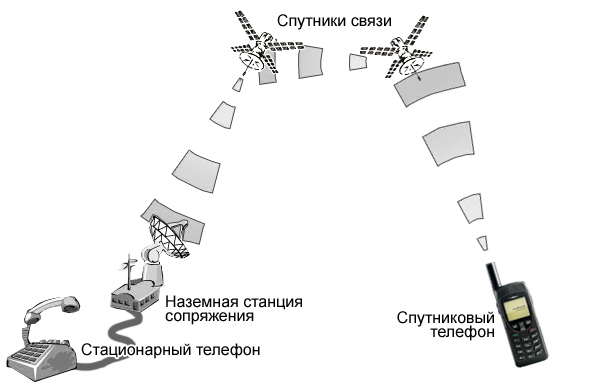
\includegraphics[scale=0.7]{70}
{\centering\caption{\newline Рис. 1.2.3.1}\\}

~

На рис. 1.2.3.1: космический сегмент - спутники связи, сигнальная часть - наземная станция сопряжения, наземный сегмент - спутниковый телефон.

\subsubsection{Преимущества и ограничения систем спутниковой связи}
Системы спутниковой связи имеют уникальные особенности, отличающие их от других систем связи. Некоторые особенности обеспечивают преимущества, делающие спутниковую связь привлекательной для ряда приложений. Другие создают ограничения, которые неприемлемы при реализации некоторых прикладных задач.

ССС имеет ряд преимуществ:
\begin{itemize}
\item Устойчивые издержки. Стоимость передачи через спутник по одному соединению не зависит от расстояния между передающей и принимающей ЗС. Более того, все спутниковые сигналы - широковещательные. Стоимость спутниковой передачи, следовательно, остается неизменной независимо от числа принимающих ЗС.
\item Широкая полоса пропускания.
\item Малая вероятность ошибки. В связи с тем, что при цифровой спутниковой передаче побитовые ошибки весьма случайны, применяются эффективные и надежные статистические схемы их обнаружения и исправления.
\end{itemize}

Выделим также ряд ограничений в использовании ССС:

\begin{itemize}
\item Значительная задержка. Большое расстояние от ЗС до спутника на геосинхронной орбите приводит к задержке распространения, длиной почти в четверть секунды. Эта задержка вполне ощутима при телефонном соединении и делает чрезвычайно неэффективным использование спутниковых каналов при неадаптированной для ССС передаче данных.
\item Размеры ЗС. Крайне слабый на некоторых частотах спутниковый сигнал, доходящий до ЗС (особенно для спутников старых поколений), заставляет увеличивать диаметр антенны ЗС, усложняя тем самым процедуру размещения станции.
\item Защита от несанкционированного доступа к информации. Широковещание позволяет любой ЗС, настроенной на соответствующую частоту, принимать транслируемую спутником информацию. Лишь шифрование сигналов, зачастую достаточно сложное, обеспечивает защиту информации от несанкционированного доступа.
\item Интерференция. Спутниковые сигналы, действующие в Ku- или Ka-полосах частот (о них ниже), крайне чувствительны к плохой погоде. Спутниковые сети, действующие в C-полосе частот, восприимчивы к микроволновым сигналам. Интерференция вследствие плохой погоды ухудшает эффективность передачи в Ku- и Ka-полосах на период от нескольких минут до нескольких часов. Интерференция в С-полосе ограничивает развертывание ЗС в районах проживания с высокой концентрацией жителей.
\end{itemize}

Влияние упомянутых преимуществ и ограничений на выбор спутниковых систем для частных сетей довольно значительно. Решение об использовании ССС, а не распределенных наземных сетей, всякий раз необходимо экономически обосновать. Все более возрастающую конкуренцию ССС составляют оптоволоконные сети связи.

\subsubsection{Космический сегмент}
Современные спутники связи, используемые в коммерческих ССС, занимают геосинхронные орбиты, в которых период орбиты равен периоду отметки на поверхности Земли. Это становится возможным при размещении спутника над заданным местом Земли на расстоянии 35800 км в плоскости экватора.

Большая высота, требуемая для поддержания геосинхронной орбиты спутника, объясняет нечувствительность спутниковых сетей к расстоянию. Длина пути от заданной точки на Земле через спутник на такой орбите до другой точки Земли в четыре раза больше расстояния по поверхности Земли между двумя ее максимально удаленными точками.

В настоящее время наиболее плотно занятая орбитальная дуга равна 76\degree \  (приблизительно 67\degree \  по 143 \degree \  западной долготы). Спутники этого сектора обеспечивают связь стран Северной, Центральной и Южной Америки.

Главными компонентами спутника являются его конструкционные элементы; системы управления положением, питания; телеметрии, трекинга, команд; приемопередатчики и антенна.

Структура спутника обеспечивает функционирование всех его компонентов. Предоставленный сам себе спутник в конечном счете перешел бы к случайным вращениям, превратившись в бесполезное для обеспечения связи устройство. Устойчивость и нужная ориентация антенны поддерживается системой стабилизации. Размер и вес спутника ограничены в основном возможностями транспортных средств, требованиями к солнечным батареям и объему топлива для жизнеобеспечения спутника (обычно в течение десяти лет).

Телеметрическое оборудование спутника используется для передачи на Землю информации о его положении. В случае необходимости коррекции положения, на спутник передаются соответствующие команды, по получении которых включается энергетическое оборудование и коррекция осуществляется.

~

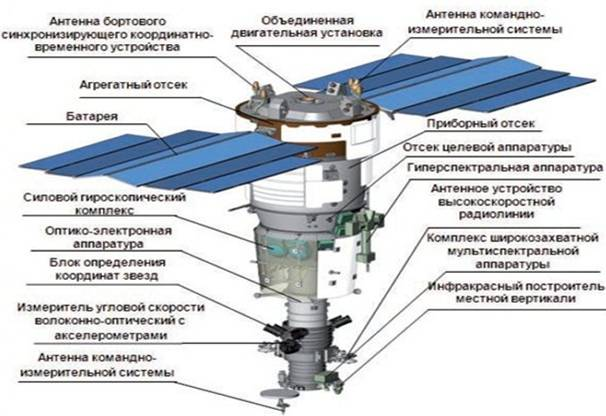
\includegraphics[scale=1.1]{71}
{\centering\caption{\newline Рис. 1.2.3.2 Cтруктура спутника}\\}

~

\subsubsection{Сигнальная часть}
Ширина полосы (bandwidth) спутникового канала характеризует количество информации, которую он может передавать в единицу времени. Типичный спутниковый приемопередатчик имеет ширину полосы 36 МГц на частотах от 4 МГц до 6 МГц.

Обычно ширина полосы спутникового канала велика. Например, один цветной телевизионный канал занимает полосу 6 МГц. Каждый приемопередатчик на современных спутниках связи поддерживает полосу в 36 МГц, при этом спутник несет 12 или 24 приемопередатчиков, что дает в результате 432 МГц или 864 МГц, соответственно.

~

Спутники связи должны преобразовывать частоту получаемых от ЗС сигналов перед ретрансляцией их к ЗС, поэтому спектр частот спутника связи выражен в парах. Из двух частот в каждой паре, нижняя используется для передачи от спутника к ЗС (нисходящие потоки), верхняя - для передачи от ЗС на спутник (восходящие потоки). Каждая пара частот называется полосой.

Современные спутниковые каналы чаще всего применяют одну из двух полос: C-полосу (от спутника к ЗС в области 6 ГГц и обратно в области 4 ГГц), или Ku-полосу (14 ГГц и 12 ГГц, соответственно). Каждая полоса частот имеет свои характеристики, ориентированные на разные задачи связи (таблица 1.2.3.1).

~

{\centering\begin{tabular}[c]{|c|c|c|c|}
\hline
Диапазоны полос \\  передачи,(GHz) & Полоса,(MHz) & Диапазон частот,(GHz) & Доступная ширина,(Hz)  \\
\hline
1.6/1.5 & 15 & 	6/4  & 	500\\
14/12 & 500 & 508.3  & 2500\\
\hline
\end{tabular}}

~

{\centering\caption{\newline Табл. 1.2.3.1 }\\}

~

Спутниковые диапозоны полос - L; полоса - C; диапозон частот - Ku; доступная ширина - Ka.

Большинство действующих спутников используют C-полосу. Передача в С-полосе может покрывать значительную область земной поверхности, что делает спутники особенно пригодными для сигналов широковещания. С другой стороны, сигналы С-полосы, являются относительно слабыми и требуют развитых и достаточно дорогих антенн на ЗС. Важная особенность сигналов С-полосы - их устойчивость к атмосферному шуму. Атмосфера земли почти прозрачна для сигналов в диапазоне 4/6 ГГц. К сожалению, этим же фактором обусловлено то, что сигналы С-полосы более всего подходят для наземных двухточечных микроволновых передач, портящих более слабые спутниковые сигналы. Данное обстоятельство заставляет размещать ЗС, использующие при передаче С-полосу, за много километров от городских центров и мест плотного проживания населения.

\subsubsection{Передача речи и данных}
Мультиплексирование с разделением частот (FDM) широко используется для мультиплексирования нескольких речевых каналов или каналов данных на один спутниковый приемопередатчик.

В FDM волновая форма каждого индивидуального телефонного сигнала фильтруется для ограничения ширины полосы диапазоном звуковых частот между 300 и 3400 Гц, затем преобразуется. Далее сигналы двенадцати каналов мультиплексируются в составной сигнал основной полосы. Каждая группа составлена из телефонных сигналов, размещенных в интервалах с шириной полосы равной 4 кГц. Затем несколько групп повторно мультиплексируются и формируют большую группу, которая может содержать от 12 до 3600 отдельных речевых каналов.

Мультиплексирование с временным разделением (TDM) - другой метод для передачи речи и/или данных по одному каналу. Если в FDM для передачи речевого сигнала (или данных) назначаются отдельные сегменты частоты внутри всей полосы, в методе TDM передача ведется по всей выделенной полосе частот. В исходящем канале повторяемые базовые временные периоды, называемые иногда фреймами (frame), разделены на фиксированное число тактов, которые выделяются последовательно для передачи сигналов входящих речевых каналов и каналов данных. Для предохранения от возможных потерь информации используются накопители (буферы).

\subsubsection{Система Aloha}
Влияние разработанного в Гавайском университете в начале 1970-х протокола множественного доступа Aloha (известного также под названием система Aloha) на развитие спутниковых и локальных сетей связи трудно переоценить.

В данной системе земные станции (ЗС) используют пакетную передачу по общему спутниковому каналу. В любой момент времени каждая ЗС может передавать лишь один пакет. Поскольку спутнику по отношению к пакетам отведена роль ретранслятора, всегда, когда пакет одной ЗС достигает спутника во время трансляции им пакета некоторой другой ЗС, обе передачи накладываются (интерферируют) и "разрушают" друг друга. Возникает требующая разрешения конфликтная ситуация.

В соответствии с ранним вариантом системы Aloha, известной под названием "чистая система Aloha", ЗС могут начать передачу в любой момент времени. Если спустя время распространения они прослушивают свою успешную передачу, то заключают, что избежали конфликтной ситуации (т.е. тем самым получают положительную квитанцию). В противном случае они знают, что произошло наложение (или, быть может, действовал какой-либо другой источник шума) и они должны повторить передачу (т.е. получают отрицательную квитанцию). Если ЗС сразу же после прослушивания повторят свои передачи, то наверняка опять попадут в конфликтную ситуацию. Требуется некоторая процедура разрешения конфликта для того, чтобы ввести случайные задержки при повторной передаче, и разнести во времени вступающие в конфликт пакеты.

Другой вариант системы Aloha состоит в разбиении времени на отрезки - окна, длина которых равна длине одного пакета при передаче (предполагается, что все пакеты имеют одну и ту же длину). Если теперь потребовать, чтобы передача пакетов начиналась только в начале окна (время привязано к спутнику), то получится двойной выигрыш в эффективности использования спутникового канала, т.к. наложения при этом ограничиваются длиной одного окна (вместо двух, как в чистой системе Aloha). \\Эта система называется синхронной системой Aloha (рис. 1.2.3.3).

~

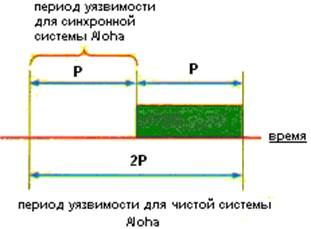
\includegraphics[scale=1.3]{72}
{\centering\caption{\newline Рис. 1.2.3.3 Период уязвимости для системы Aloha.}\\}

~

Третий подход базируется на резервировании временных окон по требованию ЗС.

Gписанная система Aloha является предшественником используемого в сетях Ethernet протокола множественного доступа с проверкой несущей и обнаружением конфликтов (CSMA-CD - Carrier Sense Multiple Access with Collision Detection). Особенность протокола CDMA-CD заключается в возможности быстрого определения конфликтов (в течение микро- и даже наносекунды) и мгновенного прекращения передачи. На спутниковых каналах из-за большого времени распространения оперативное прекращение передачи заведомо испорченных пакетов, к сожалению, невозможно.

Другим усовершенствованием системы Aloha может служить назначение приоритетов для ЗС с большой интенсивностью нагрузки.

\subsubsection{Наземный сегмент}
Технологическое развитие привело к значительному уменьшению размеров ЗС. На начальном этапе спутник не превышал нескольких сотен килограммов, а ЗС представляли собой гигантские сооружения с антеннами более 30 м в диаметре. Современные спутники весят несколько тонн, а антенны, зачастую не превышающие 1 м в диаметре, могут быть установлены в самых разнообразных местах. Тенденция уменьшения размеров ЗС вместе с упрощением установки оборудования приводит к снижению его стоимости. На сегодняшний день стоимость ЗС является, пожалуй, главной характеристикой, определяющей широкое распространение ССС. Преимущество спутниковой связи основано на обслуживании географически удаленных пользователей без дополнительных расходов на промежуточное хранение и коммутацию. Любые факторы, понижающие стоимость установки новой ЗС, однозначно содействуют развитию приложений, ориентированных на использование ССС.
\newpage Относительно высокие издержки развертывания ЗС позволяют наземным волоконно-оптическим сетям в ряде случаев успешно конкурировать с ССС.

Следовательно, главное преимущество спутниковых систем состоит в возможности создавать сети связи, предоставляющие новые услуги связи или расширяющие прежние, при этом с экономической точки зрения преимущество ССС обратно пропорционально стоимости ЗС.

В зависимости от типа, ЗС имеет возможности передачи и/или приема. Как уже отмечалось, фактически все интеллектуальные функции в спутниковых сетях осуществляются в ЗС. Среди них - организация доступа к спутнику и наземным сетям, мультиплексирование, модуляция, обработка сигнала и преобразование частот. Отметим, наконец, что большинство проблем в спутниковой передаче решается оборудованием ЗС.

~

В настоящее время выделяются четыре типа ЗС. Наиболее сложными и дорогостоящими являются ориентированные на большую интенсивность пользовательской нагрузки ЗС с очень высокой пропускной способностью. Станции такого типа предназначены для обслуживания пользовательских популяций, требующих для обеспечения нормального доступа к ЗС волоконно-оптических линий связи. Подобные ЗС стоят миллионы долларов.

Станции средней пропускной способности эффективны для обслуживания частных сетей корпораций. Размеры подобных сетей ЗС могут быть самыми разнообразными в зависимости от реализованных приложений (передача речи, видео, данных). Различаются два типа корпоративных ССС.

Развитая корпоративная ССС с большими капиталовложениями обычно поддерживает такие услуги, как видеоконференция, электронная почта, передача видео, речи и данных. Все ЗС такой сети имеют одинаково большую пропускную способность, а стоимость станции доходит до 1 миллиона долларов.

Менее дорогостоящим типом корпоративной сети является ССС большого числа (до нескольких тысяч) микротерминалов (VSAT - Very Small Aperture Terminal) связанных с одной главной ЗС (MES - Master Earth Station). Данные сети ограничиваются обычно приемом/передачей данных и приемом аудио-видеоуслуг в цифровом виде. Микротерминалы общаются между собой посредством транзита с обработкой через главную ЗС. Топология таких сетей является звездообразной.

Четвертый тип ЗС ограничен возможностями приема. Это самый дешевый вариант станции, поскольку ее оборудование оптимизируется под предоставление одной или нескольких конкретных услуг. Данная ЗС может быть ориентирована на прием данных, аудиосигнала, видео или их комбинаций.

~

Последние достижения технологии в области спутниковой связи говорят о больших потенциальных возможностях ССС в расширении пропускной способности каналов передачи, разработке и внедрении новых служб связи. Будущее ССС за широкополосными широковещательными приложениями и спутниковыми системами подвижной связи.


\subsection{Передача аудиоданных черз интернет}
Интернет давно и уверенно трансформируется в направлении от коммуникационной среды для обмена данными среди ученых и специалистов к прообразу мировой коммуникационной мультимедийной супермагистрали, одинаково пригодной в качестве среды для множества видов профессиональной деятельности и бизнес-применений, включая такие виды массового обслуживания, как торговля, информационная и развлекательная индустрия, средства массовой информации.

Разработчики аппаратно-программных приложений к ПЭВМ давно уже прошли этап освоения мультимедиа-функций для отдельно стоящих персональных компьютеров и компьютеров в локальных вычислительных сетях. Теперь многие сосредоточили свои усилия на передаче аудио- и видеоданных в режиме реального времени в компьютерных сетях. 

\subsubsection{Компьютерная телефония}
Самой заметной из последних новинок звуковых коммуникаций в Интернете является ПО, позволяющее географически удаленным пользователям устанавливать телефонную связь через Интернет и платить за нее намного меньше, чем за такой же звонок по обычным телефонным линиям. Попросту говоря, шлюз способен соединить обыкновенный телефон с сетью Интернет. Но данные могут поступать и из других источников. В теории ограничений на способ связи нет: вы можете воспользоваться компьютером (если общаются два компьютера, иногда можно обойтись вовсе без шлюза), обыкновенным телефоном, радиопередатчиком и т.п.

В общем виде схема связи выглядит так:

~

Абонент 1 -> [локальная телефонная сеть 1] -> [шлюз 1] -> \\ -> Интернет -> [шлюз 2] -> [локальная телефонная сеть 2] -> Абонент 2.

~

Ключевым элементом интернет-телефонии является связка шлюз-Интернет. Шлюз представляет собой компьютер-сервер, дополненный специальными платами расширения и соответствующим программным обеспечением. Он служит интерфейсом между передающим звук устройством пользователя (телефоном, компьютером и т.п.) и сетью Ин-тернет. Шлюз обеспечивает прием и преобразование данных в форму, удобную для пере-сылки по Сети (и обратное преобразование). Абоненту всего лишь нужно связаться с ним тем или иным способом. Шлюз, имеющий выход в Интернет, передаст по Сети данные на другой такой же шлюз, ближайший к абоненту номер 2, после чего, претерпев обратное преобразование, звук достигнет цели своего путешествия.

Интернет-телефония иначе называется IP-телефонией.

\newpage
\subsubsection{Варианты использования IP-телефонии}
\begin{enumerate}
\item) Компьютер - компьютер

\par Два компьютера, подключенные к сети Интернет, могут общаться без посредников. Из общей схемы исчезнет шлюз, поскольку необходимость преобразования сигнала отпала (если быть более точным, в качестве шлюза выступает некая программа - интернет-телефон, запущенная на обоих компьютерах). Данные сразу передаются по стандартным протоколам Интернета, поэтому помехи проникнуть в пакет данных не могут. Единствен-ное негативное воздействие помех - задержка пакетов. Неудивительно, что именно задержки являются главной проблемой интернет-телефонии. Причин их возникновения несколько. Одни связаны с принципом построения сетей TCP/IP и особенностями коммутации пакетов, другие зависят от общей загрузки сети, качества линии связи и скорости модема. Если задержка превышает 250 миллисекунд, она становится заметной. Поскольку программа не контролирует контекст передаваемого разговора, паузы вклиниваются в беседу случайным образом - чаще на полуслове. Окончание слова возникает в наушниках или колонках после секундного затишья. Повлиять на качество звука можно, лишь купив более быстрый модем и выбрав провайдера с мощными каналами связи.






\end{enumerate}

























\end{document}





